\chapter{Job 33}

\begin{figure}
  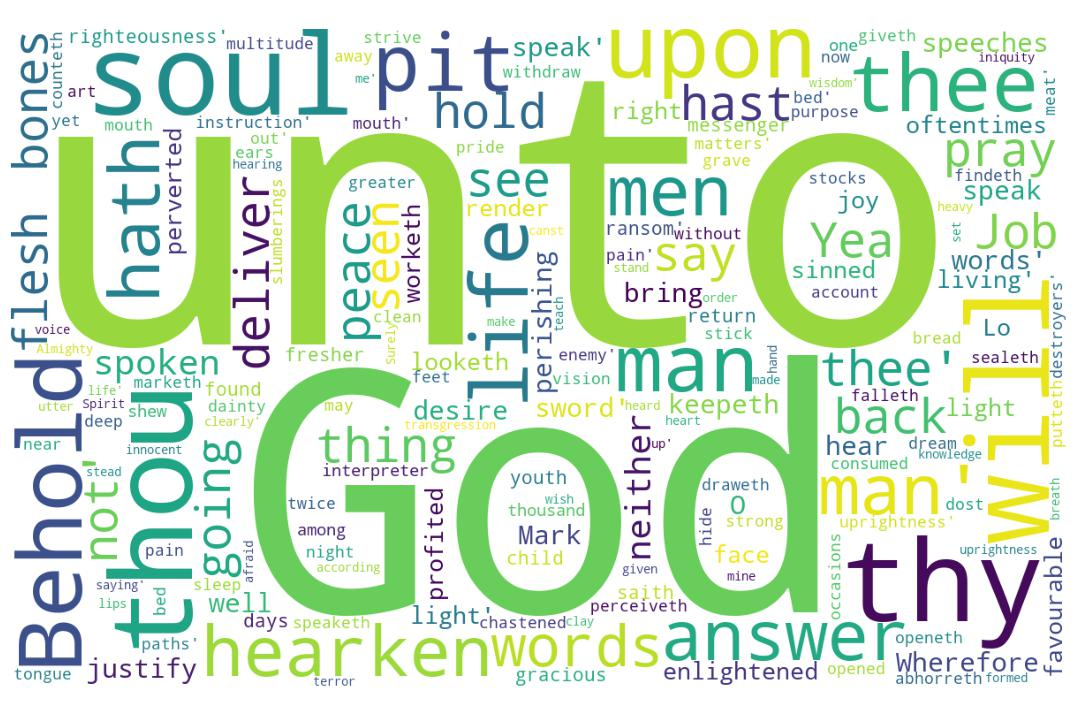
\includegraphics[width=\linewidth]{18OT-Job/Job33-WordCloud.jpg}
  \caption{Job 33 Word Cloud}
  \label{fig:Job 33 word Cloud}
\end{figure}

\marginpar{\scriptsize \centering \fcolorbox{bone}{lime}{\textbf{ELIHU THE MEDIATOR}}\\ (Job 33:1-33) \begin{compactenum}[I.][8]
    \item Elihu has a \textbf{Message}  \index[scripture]{Job!Job 33:01}(Job 33:1, \index[scripture]{Job!Job 33:23}Job 33:23)
    \item Elihu is acting as the \textbf{Mediator}  \index[scripture]{Job!Job 33:06}(Job 33:6)
    \item Speaks of Job's \textbf{Misperception}  \index[scripture]{Job!Job 33:12}(Job 33:12)
    \item Speaks of the place of \textbf{Man}  \index[scripture]{Job!Job 33:12}(Job 33:12)    \item God's \textbf{Mercy} to reveal any truth \index[scripture]{Job!Job 33:24}(Job 33:24)
    \item Speaks of the Redemption of \textbf{Man}  \index[scripture]{Job!Job 33:29}(Job 33:29)
\end{compactenum}}

\footnote{\textcolor[cmyk]{0.99998,1,0,0}{\hyperlink{TOC}{Return to end of Table of Contents.}}}\footnote{\href{https://www.audioverse.org/english/audiobibles/books/ENGKJV/O/Job/1}{\textcolor[cmyk]{0.99998,1,0,0}{Job  Audio}}}\textcolor[cmyk]{0.99998,1,0,0}{Wherefore, Job,  \fcolorbox{bone}{bone}{I} pray thee, hear my speeches, and hearken to all \fcolorbox{bone}{lime}{my} \fcolorbox{bone}{lime}{words}.} %\fcolorbox{bone}{lime}{my}
[2] \textcolor[cmyk]{0.99998,1,0,0}{Behold, now  \fcolorbox{bone}{bone}{I} have opened my mouth, my tongue hath spoken in my mouth.}
[3] \textcolor[cmyk]{0.99998,1,0,0}{My words \emph{shall} \emph{be} \emph{of} the uprightness of my heart: and my lips shall utter knowledge clearly.}
[4] \textcolor[cmyk]{0.99998,1,0,0}{The Spirit of God hath made me, and the breath of the Almighty hath given me life.}
[5] \textcolor[cmyk]{0.99998,1,0,0}{If thou canst answer me, set \emph{thy} \emph{words} in order before me, stand up.}
[6] \textcolor[cmyk]{0.99998,1,0,0}{Behold,  \fcolorbox{bone}{bone}{I} \emph{am} according to thy wish \fcolorbox{bone}{lime}{in God's stead}:  \fcolorbox{bone}{bone}{I} also am formed out of the clay.}
[7] \textcolor[cmyk]{0.99998,1,0,0}{Behold, my terror shall not make thee afraid, neither shall my hand be heavy upon thee.}
[8] \textcolor[cmyk]{0.99998,1,0,0}{Surely thou hast spoken in mine hearing, and  \fcolorbox{bone}{bone}{I} have heard the voice of \emph{thy} words, \emph{saying},}
[9] \textcolor[cmyk]{0.99998,1,0,0}{ \fcolorbox{bone}{bone}{I} am clean without \fcolorbox{bone}{MYGOLD}{transgression},  \fcolorbox{bone}{bone}{I} \emph{am} innocent; neither \emph{is} \emph{there} iniquity in me.}
[10] \textcolor[cmyk]{0.99998,1,0,0}{Behold, he findeth occasions against me, he counteth me for his enemy,}
[11] \textcolor[cmyk]{0.99998,1,0,0}{He putteth my feet in the stocks, he marketh all my paths.}
[12] \textcolor[cmyk]{0.99998,1,0,0}{Behold, \fcolorbox{bone}{lime}{\emph{in} this} thou art not just:  \fcolorbox{bone}{bone}{I} will answer thee, that God is greater than \fcolorbox{bone}{lime}{man}.}
[13] \textcolor[cmyk]{0.99998,1,0,0}{Why dost thou strive against him? for he giveth not account of any of his matters.}
[14] \textcolor[cmyk]{0.99998,1,0,0}{For God speaketh once, yea twice, \emph{yet} \emph{man} perceiveth it not.}
[15] \textcolor[cmyk]{0.99998,1,0,0}{In a dream, in a vision of the night, when deep sleep falleth upon men, in slumberings upon the bed;}
[16] \textcolor[cmyk]{0.99998,1,0,0}{Then he openeth the ears of men, and sealeth their instruction,}
[17] \textcolor[cmyk]{0.99998,1,0,0}{That he may withdraw man \emph{from} \emph{his} purpose, and hide pride from man.}
[18] \textcolor[cmyk]{0.99998,1,0,0}{He keepeth back his soul from the pit, and his life from perishing by the sword.}
[19] \textcolor[cmyk]{0.99998,1,0,0}{He is chastened also with pain upon his bed, and the multitude of his bones with strong \emph{pain}:}
[20] \textcolor[cmyk]{0.99998,1,0,0}{So that his life abhorreth bread, and his soul dainty meat.}
[21] \textcolor[cmyk]{0.99998,1,0,0}{His flesh is consumed away, that it cannot be seen; and his bones \emph{that} were not seen stick out.}
[22] \textcolor[cmyk]{0.99998,1,0,0}{Yea, his soul draweth near unto the grave, and his life to the destroyers.}
[23] \textcolor[cmyk]{0.99998,1,0,0}{If there be a messenger with him, an interpreter, one among a thousand, to shew unto man his uprightness:}
[24] \textcolor[cmyk]{0.99998,1,0,0}{Then he is \fcolorbox{bone}{lime}{gracious} unto him, and saith, Deliver him from going down to the pit:  \fcolorbox{bone}{bone}{I} have found a ransom.}
[25] \textcolor[cmyk]{0.99998,1,0,0}{His flesh shall be fresher than a child's: he shall return to the days of his youth:}
[26] \textcolor[cmyk]{0.99998,1,0,0}{He shall pray unto God, and he will be favourable unto him: and he shall see his face with joy: for he will render unto man his \fcolorbox{bone}{MYGOLD}{righteousness}.}
[27] \textcolor[cmyk]{0.99998,1,0,0}{He looketh upon men, and \emph{if} \emph{any} say,  \fcolorbox{bone}{bone}{I} have sinned, and perverted \emph{that} \emph{which} \emph{was} right, and it profited me not;}
[28] \textcolor[cmyk]{0.99998,1,0,0}{He will deliver his soul from going into the pit, and his life shall see the light.}
[29] \textcolor[cmyk]{0.99998,1,0,0}{Lo, all these \emph{things} worketh God oftentimes with \fcolorbox{bone}{lime}{man},}
[30] \textcolor[cmyk]{0.99998,1,0,0}{To bring back his soul from the pit, to be enlightened with the light of the living.}
[31] \textcolor[cmyk]{0.99998,1,0,0}{Mark well, O Job, hearken unto me: hold thy peace, and  \fcolorbox{bone}{bone}{I} will speak.}
[32] \textcolor[cmyk]{0.99998,1,0,0}{If thou hast any thing to say, answer me: speak, for  \fcolorbox{bone}{bone}{I} desire to justify thee.}
[33] \textcolor[cmyk]{0.99998,1,0,0}{If not, hearken unto me: hold thy peace, and  \fcolorbox{bone}{bone}{I} shall teach thee wisdom.}